\subsection{Research Objectives and Anticipated Results}

\begin{figure}[t]
    \centering
%    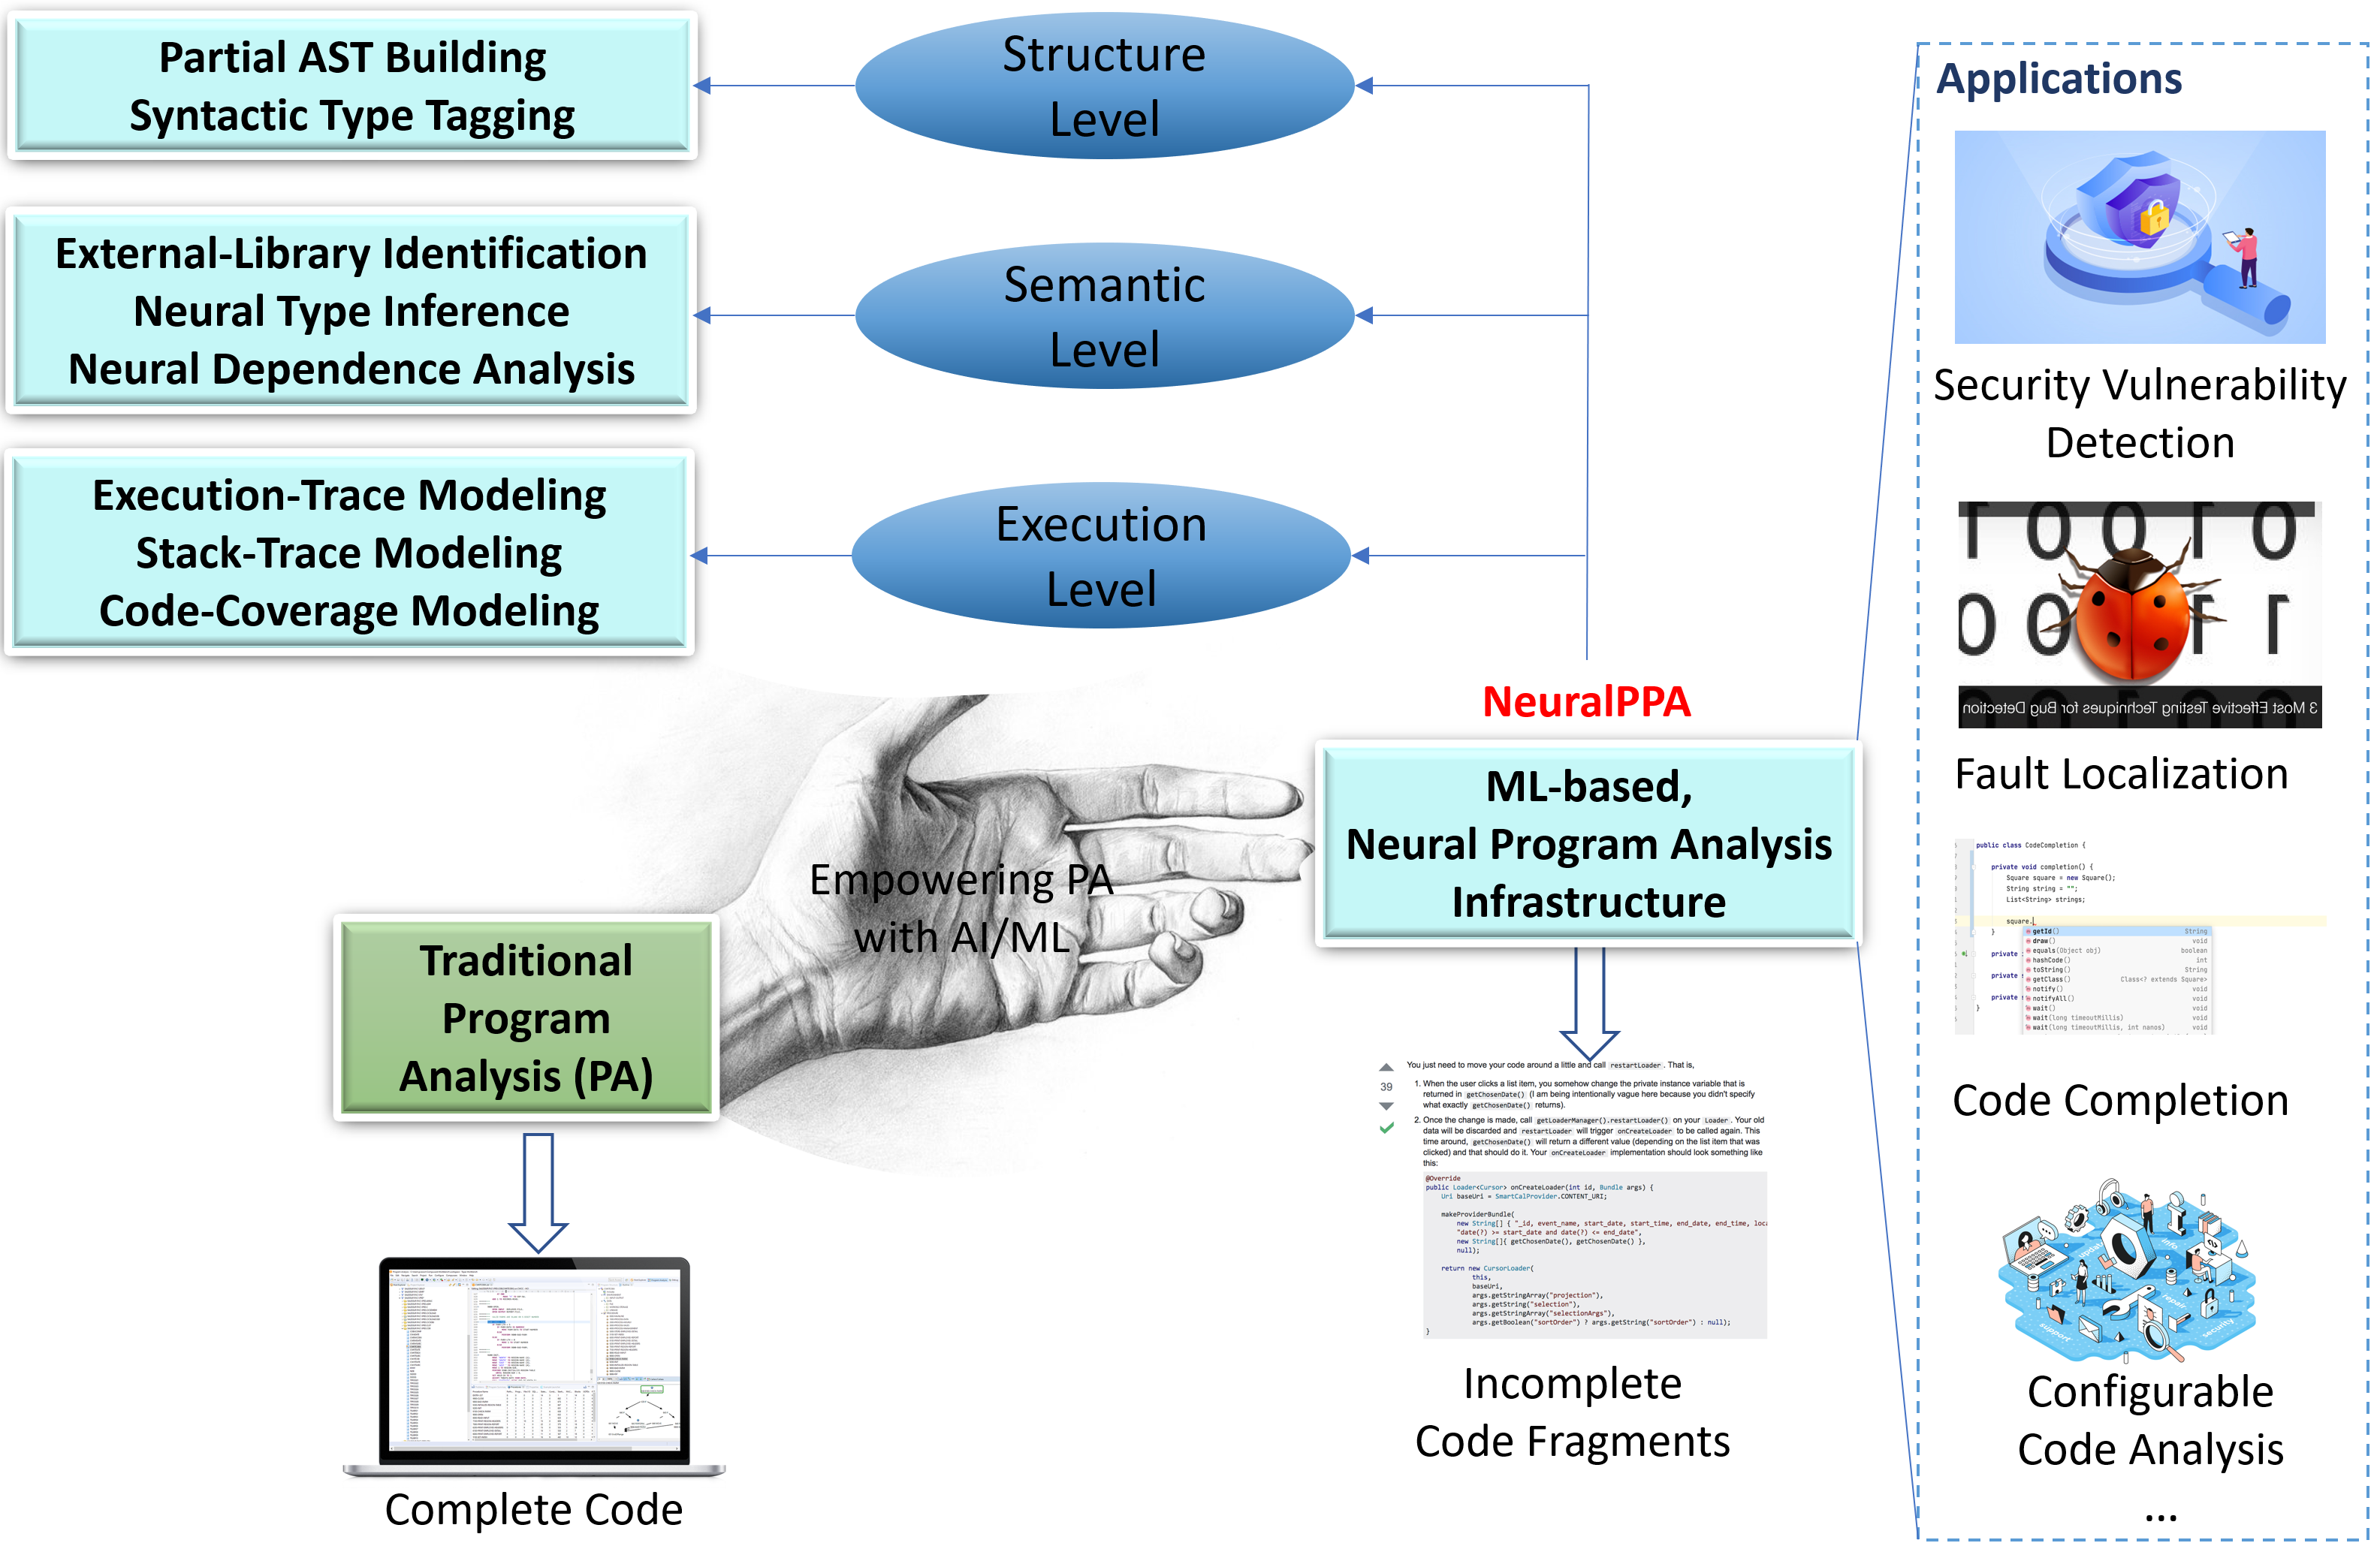
\includegraphics[width=0.83\textwidth]{graphs/neuralppa}
%    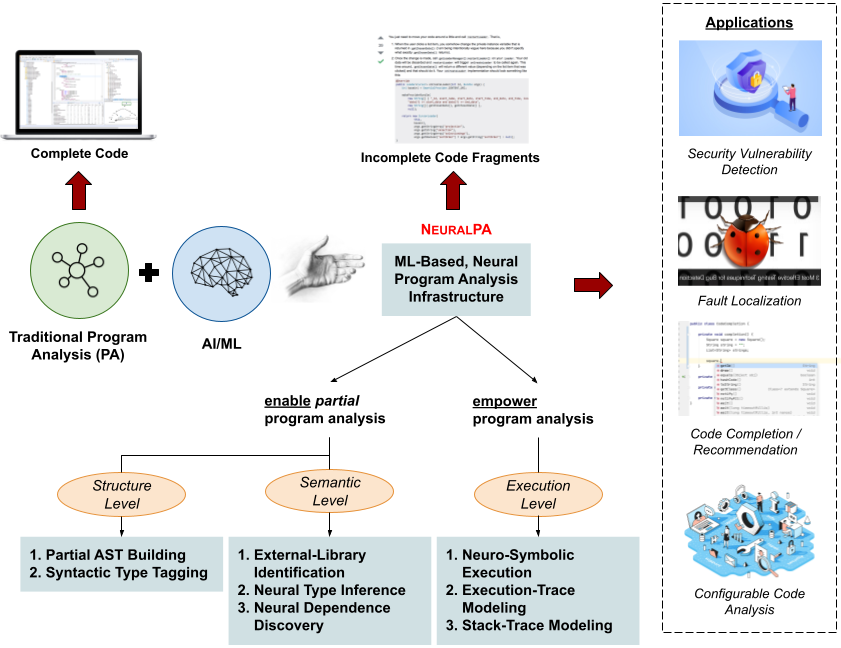
\includegraphics[width=0.92\textwidth]{figures/infra-design-3.png}
    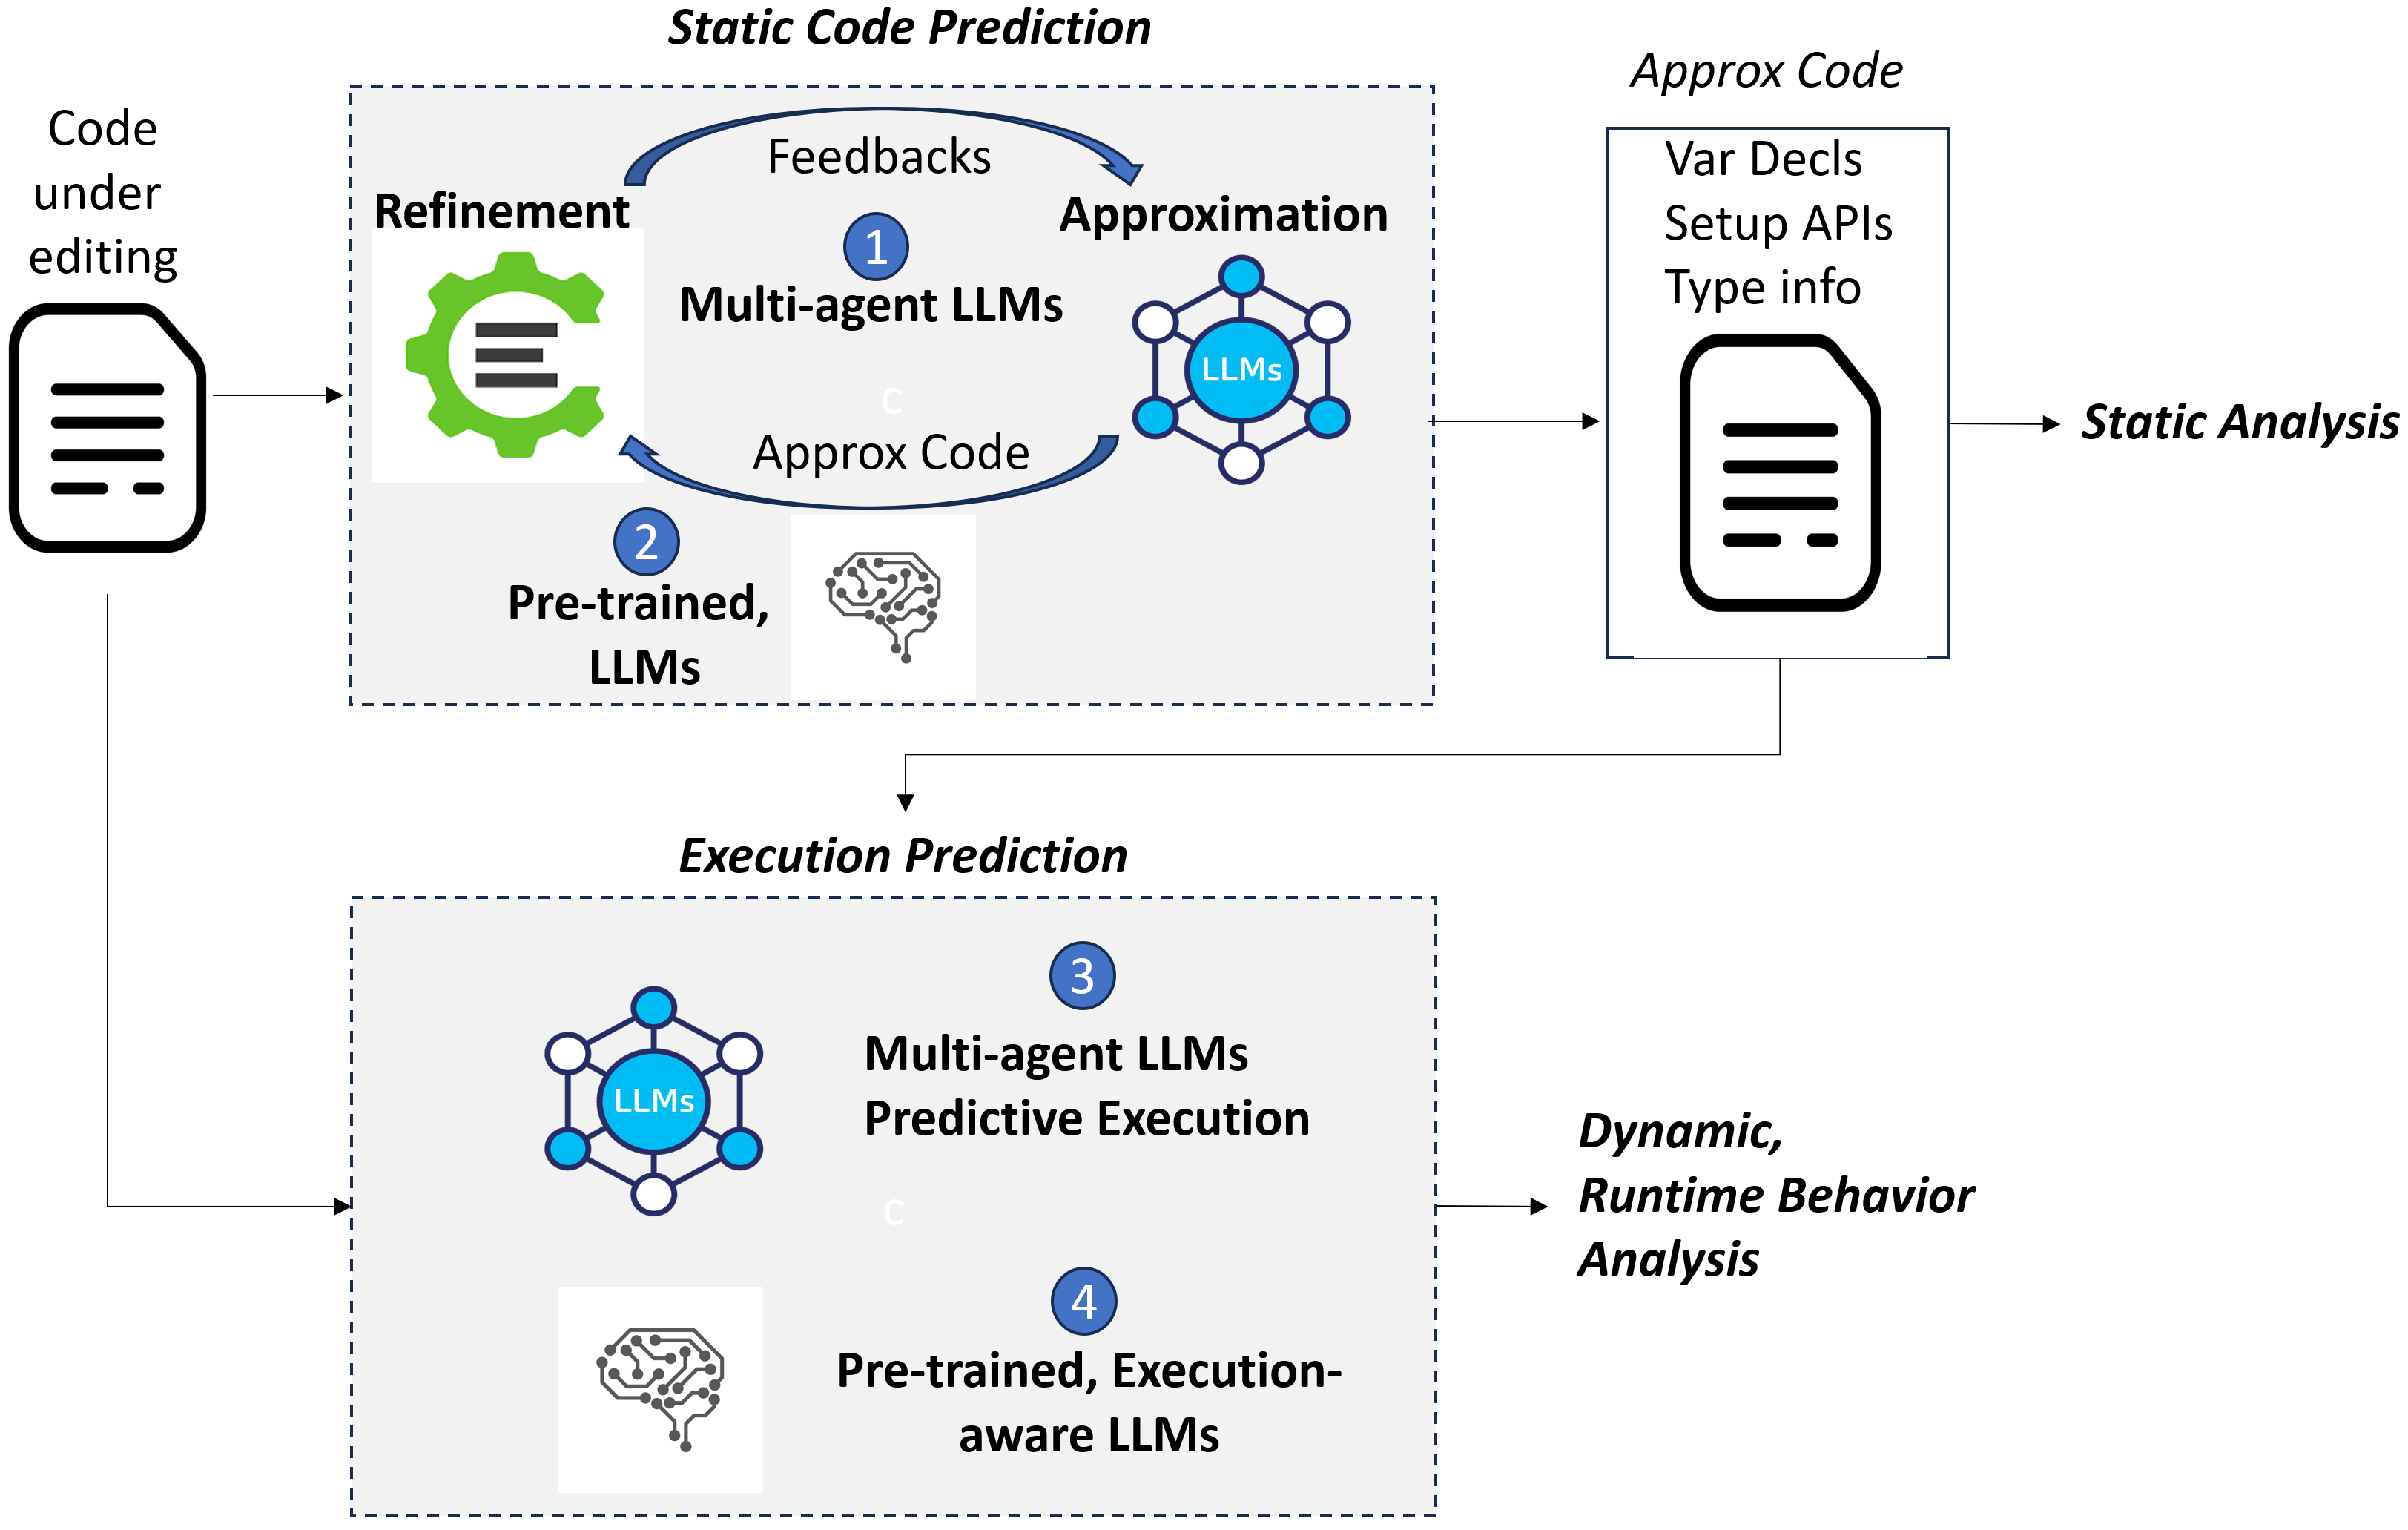
\includegraphics[width=0.92\textwidth]{overview.png}
    \vspace{-10pt}
    \caption{Predictive Program Analysis: Learning to Analyze Program Behaviors for Incomplete Code}
    \label{fig:arch}
\end{figure}


In this proposal, we seek to advance the state-of-the-art in
traditional program analysis by means of {\tool}, a Predictive Program
Analysis framework, with the goal to support program analysis for
incomplete/inexecutable code. We aim to establish {\em a scientific
  foundation, novel methodologies, frameworks, models, and algorithmic
  solutions for predictive program analysis} with the following focus
areas:



(1) {\bf enabling static program analysis on incomplete code}, and

(2) {\bf supporting predictive analysis for dynamic program behaviors}.

%\noindent Figure~\ref{fig:arch} illustrates the framework for {\tool},
%which will allow the construction of efficient program analysis
%techniques for (partial) code, also based on which downstream vulnerability detection and assessment applications can be built.

The key philosophy that drives our work is that the analysis of
partial code can be learned from the analysis of entire programs in
the wealth of information obtained from ultra-large-scale, open-source
software repositories. To accomplish these tasks, we propose the
following thrusts of research in {\tool} (Figure~\ref{fig:arch}):

\noindent \textbf{Thrust 1. Neural Structural Analysis Infrastructure.} ({\em Section~\ref{sec:thrust1}})
One of the key foundations of {\tool} lies in its neural structural analysis component, which is built upon the well-defined structure and semantics of source code. This component serves two primary functions. Firstly, it draws upon the syntactic structures of comprehensive code samples from large-scale repositories in the training dataset. From this data, it constructs an abstract syntax tree (AST) that best encapsulates the syntactic arrangement of the provided partial code, aiming for the highest likelihood or probability. In contrast, existing program-analysis-based partial parsing methods~\cite{ppa08} rely on heuristics derived from the syntactic rules of programming languages, lacking the capacity to rank or score potential candidates. The second task of this component involves labeling code tokens with the corresponding types of syntactic units, encompassing statement types (\code{if}, \code{for}, etc.), variables, fields, methods, classes, and more. Both tasks can be efficiently executed through our dual-learning-based approaches.

%Source code has a well-defined structure and semantics. Thus, the basic infrastructure in {\tool} is the neural structural analysis component, which primarily has two tasks. First, it learns from the syntactic structures of the complete code in the training dataset collected from large-scale code repositories, to derive the abstract syntax tree (AST) that best represents the syntactic structure of the given partial code, i.e., with the highest likelihood/probability. The existing program-analysis-based partial parsing approaches~\cite{ppa08} rely on the heuristics on the syntactic rules of the programming languages. They do not give us any ranking or scores among the potential candidates. The second task of this component is to tag the code tokens with the types of the syntactic units including the statement types (\code{if}, \code{for}, etc.), variables, fields, methods, classes, etc. Both of the tasks can be performed with our learning-based approaches in a dual-learning manner.
  
\vspace{3pt}
\noindent \textbf{Thrust 2. Neural Semantic Analysis Infrastructure.}
({\em Section~\ref{sec:thrust2}}) The basis components for several
analysis techniques on the semantics of the program could tentatively
include the following (more components will be added as the project
evolves):

1) the identification of the APIs of the external libraries in the
external references in the partial code: this is needed because the
partial code contains the undeclared reference and/or
declaration/reference ambiguity without explicit declaration of the
APIs in the external libraries. The knowledge on the external
libraries enables more precise analysis of the code snippets.

2) the inference of the type information for the entities in the
partial code: due to the ambiguity in the declaration, the types of
the variables and statements are not always obviously
identified. Thus, the type inference is a basic service within
{\tool}.

3) the inference of the program dependencies among the statements in
the partial code: several program analysis techniques are based on the
program dependencies, which are not always obtainable due to the
incompleteness of the given code fragment.

4) Program slicing: program slices are important in both code
understanding and program analysis for code snippets. That allows the
analysis on the statements affecting or to be affected by a specified
variable. All traditional program slicing techniques require the code
to be complete.

\vspace{3pt}
\noindent \textbf{Thrust 3. Predictive Execution.}  ({\em
  Section~\ref{sec:thrust3}}) We advocate for an execution paradigm
called predictive execution. In predictive execution, with a specific
input, the execution is not carried out with the computer performing
the instruction in the program. Instead, a trained machine learning
model predicts the execution steps and as a result, the execution
trace corresponding to the input is derived without actual execution.
The predictive execution paradigm has the potential to improve
efficiency and effectiveness in software testing, fault localization,
and software vulnerability detection.

%Symbolic execution is a means of analyzing a program to determine what
%inputs cause each part of a program to execute. Symbolic execution
%performs executing a program abstractly, so that one abstract
%execution covers multiple possible inputs, which are assumed to have
%symbolic values. We aim to explore the novel area in AI named
%neuro-symbolic learning, which seeks to combine traditional
%rules-based AI approaches with modern deep learning techniques.  We
%will leverage traditional program analysis rules to enhance the
%learning of the characteristics on the execution of the partial code
%fragment.

\vspace{3pt}
\noindent \textbf{Thrust 4. Neural Partial Program Analysis
  Applications.}  ({\em Section~\ref{sec:thrust4}}) Our last thrust of
research is aimed to evaluate our partial program analysis
infrastructure in vulnerability detection for code snippets.
%2) fault localization, and 3) code completion.

%\vspace{3pt}
%\noindent \textbf{Thrust ???. Neural Execution Analysis Infrastructure.}
%({\em Section~\ref{}}) All the dynamic analysis techniques require the
%analysis and understanding of the execution. However, for an
%incomplete code, we first need to design a component that can wrap
%around the given code fragment with the minimum code so that the code
%fragment can be executed. When the code is executed, we also need the
%approaches that represent the executed statements and their relations,
%model the execution and stack traces, and model the code coverages
%for an execution.




Toward this theme, in our preliminary work, we developed DeepPDA
(Section~\ref{sec:deeppda}), a neural network-based partial program
dependence analysis approach that learns to derive the program
dependencies for any code fragments (i.e., both complete and
incomplete). In our preliminary empirical evaluation, we intrinsically
evaluated it on Java and C/C++ programs. We trained DeepPDA on
complete code. For testing, we treated each method individually and
chose a consecutive portion within the method to predict the program
dependencies, and compared them against the actual
dependencies. Overall, DeepPDA predicts CFGs/PDGs in Java with
an F-score of 94.29\%, and in C++ with an F-score of 92.46\%. As
another preliminary work (Section~\ref{sec:statype}), we also
developed an approach to derive the data types of the variables in the
code snippets. We treat the problem as statistical machine translation
from source code with partially qualified names to source code with
full names. Our preliminary evaluation on StackOverflow posts shows
that our technique achieves high accuracy with 97.6\% precision and
96.7\% recall in deriving data types in code snippets.

We also test the usefulness of the PDGs predicted by DeepPDA (i.e.,
PDG*) on the downstream task of method-level vulnerability
detection. We discover that the performance of the vulnerability
detection tool utilizing PDG* is only 1.1\% less than that utilizing
the PDGs generated by a program analysis tool.
%Furthermore, we report 
We also report the detection of 14 real-world vulnerable code snippets
from StackOverflow by a learning-based vulnerability detection
tool that employs the PDGs predicted by DeepPDA for these code snippets.

\begin{table*}[t]
	\vspace{-15pt}
\begin{center}
{\footnotesize{
\begin{tabular}{cc}
\begin{tabular}[t]{|p{0.2in}|p{2.95in}|} 
\hline
\multicolumn{2}{|>{\columncolor[gray]{0}}c|}{\textcolor{white}
{\bf Year 1 Project Milestones \& Deliverables}}\\
\hline 
\hline
\multicolumn{2}{|c|}{\bf T1. Neural Structure Analysis Infrastructure}\\
\hline
{\bf 1.1} & Neural Syntactic Type Tagging\\
{\bf 1.2} & Neural Partial AST Building\\
{\bf 1.3} & Evaluation of the components\\
\hline
\hline
\multicolumn{2}{|c|}{\bf T2. Neural Semantic Analysis Infrastructure}\\ 
\hline
{\bf 2.1} & External-Library Identification\\
\hline
%\hline
%\multicolumn{2}{|c|}{\bf Integrate Code Synthesis into Tools}\\
%\hline
%{\bf 1.5} & \goalOneFour.\\
%\hline
\multicolumn{2}{c}{}
\end{tabular}
&
\begin{tabular}[t]{|p{0.2in}|p{2.95in}|} \hline
\multicolumn{2}{|>{\columncolor[gray]{0}}c|}{\textcolor{white}
{\bf Year 2 Project Milestones \& Deliverables}}\\
\hline 
\hline
\multicolumn{2}{|c|}{\bf T2. Neural Semantic Analysis Infrastructure}\\
\hline
{\bf 2.2} & Neural Type Inference\\
{\bf 2.3} & Neural Dependence Analysis\\
%{\bf 2.3} & Integrate Evaluation Framework into Design Environment\\
%{\bf 2.4} & Evaluate CRL Framework with Existing Models\\
%{\bf 2.3} & \goalTwoThree.\\

\hline
\hline
\multicolumn{2}{|c|}{\bf T3. Neural Execution Analysis}\\ 
\hline
%{\bf 3.1} & Design New Code Representations and Learning Models.\\
{\bf 3.1} & Neural Execution-Trace Modeling\\
%{\bf 2.4} & Advance FL and RT-CI Approaches.\\
%{\bf 2.5} & Advance Regression Testing in CI Approaches.\\
%{\bf 2.5} & Advance APR Approaches with Framework.\\
\hline
%\hline
%\multicolumn{2}{|c|}{\bf Community Involvement: Capacity Building}\\
%\hline
%{\bf 2.4} & \goalTwoFour.\\
%{\bf 2.5} & \goalTwoFive.\\
%{\bf 2.6} & \goalTwoSix.\\
%\hline
\multicolumn{2}{c}{}
\end{tabular}
\end{tabular}\\
\vspace*{-.3cm}
\begin{tabular}{c}\hline
\multicolumn{1}{|>{\centering\columncolor[gray]{0}}p{6.44in}|}{\textcolor{white}
{\bf Year 3 Project Milestones \& Deliverables}}\\
\hline
\end{tabular}\\
\vspace*{-.2cm}
\begin{tabular}{cc}
\begin{tabular}[t]{|p{0.2in}|p{2.95in}|}
\hline
\multicolumn{2}{|c|}{\bf T3. Neural Execution Analysis}\\
\hline
{\bf 3.2} & Neural Stack Trace Modeling\\
{\bf 3.3} & Neural Code Coverage Modeling\\

%{\bf 3.3} & Testing on Models in IDE tools.\\
\hline
%\hline
%\multicolumn{2}{|c|}{\bf \goalTwo}\\ 
%\hline
%{\bf 3.3} & \goalThreeThree.\\
%\hline
\multicolumn{2}{c}{}
\end{tabular}
&
\begin{tabular}[t]{|p{0.2in}|p{2.95in}|}
\hline
\multicolumn{2}{|c|}{\bf T4. Neural Partial Program Analysis Applications}\\
\hline
%{\bf 3.1} & Design New Code Representations\\

{\bf 4.1} & Security Vulnerablity Detection with {\tool}\\
{\bf 4.2} & Fault Localization and Completion with {\tool}\\

\hline
\multicolumn{2}{c}{}
\end{tabular}
\end{tabular}
\vspace{-15pt}
}}
\end{center}
\vspace*{-.3in}
%\caption{Tasks and Milestones. (Rep. = Representation)}
\caption{The 3-year schedule of Thrusts, Tasks, and Milestones of this proposal.}
%the schedule of Thrusts, Tasks, and Milestones of this proposal.
%\vspace{-10pt}
\label{tab:milestones}
\vspace{-10pt}
\end{table*}
%

